%% Patent Application: Computer-Implemented Method for Computing Protein Folding
%% Jamming Frequency from First Principles
%% Inventor: Jonathan Washburn
%% Contact: washburn.jonathan@gmail.com
%% Filing Date: January 2026

\documentclass[12pt,letterpaper]{article}

\usepackage[margin=1in]{geometry}
\usepackage{amsmath,amssymb,amsfonts}
\usepackage{graphicx}
\usepackage{tikz}
\usetikzlibrary{shapes,arrows,positioning,calc}
\usepackage{booktabs}
\usepackage{array}
\usepackage{enumitem}
\usepackage{fancyhdr}
\usepackage{xcolor}
\usepackage{hyperref}
\usepackage{setspace}
\usepackage{listings}

% Patent-style formatting
\setlength{\parindent}{0.5in}
\setlength{\parskip}{0.5em}
\onehalfspacing

% Header
\pagestyle{fancy}
\fancyhf{}
\rhead{Patent Application}
\lhead{Washburn}
\rfoot{Page \thepage}

\hypersetup{
    colorlinks=true,
    linkcolor=blue,
    urlcolor=blue,
    citecolor=blue
}

% Code listing style
\lstset{
    basicstyle=\ttfamily\small,
    breaklines=true,
    frame=single,
    numbers=left,
    numberstyle=\tiny,
    keywordstyle=\color{blue},
    commentstyle=\color{green!50!black},
    stringstyle=\color{red!70!black},
    showstringspaces=false
}

% Custom colors
\definecolor{compute}{RGB}{100,150,200}
\definecolor{output}{RGB}{200,150,100}
\definecolor{validate}{RGB}{100,200,150}

\begin{document}

%% ============================================================================
%%                              TITLE PAGE
%% ============================================================================

\begin{center}
\vspace*{0.8in}

{\LARGE \textbf{PATENT APPLICATION}}

\vspace{0.4in}

{\Large \textbf{COMPUTER-IMPLEMENTED METHOD FOR}}

{\Large \textbf{COMPUTING PROTEIN FOLDING JAMMING}}

{\Large \textbf{FREQUENCY FROM FIRST PRINCIPLES}}

\vspace{0.8in}

\textbf{PROVISIONAL PATENT APPLICATION}

\vspace{0.5in}

\begin{tabular}{ll}
\textbf{Inventor:} & Jonathan Washburn \\
\textbf{Email:} & washburn.jonathan@gmail.com \\
\textbf{Filing Date:} & January 17, 2026 \\
\textbf{Application Type:} & Utility Patent (Provisional) \\
\textbf{Related Applications:} & Patents 001--003 (Method, Apparatus, Verification) \\
\end{tabular}

\vspace{0.8in}

\textit{A computer-implemented method for calculating the optimal frequency for modulating protein folding rates based on the golden ratio ($\varphi$) timescale ladder, including generation of operating setpoints, frequency sweep windows, isotope-shifted frequencies, and acceptance criteria for experimental validation.}

\vfill

\textbf{CONFIDENTIAL --- PATENT PENDING}

\end{center}

\newpage

%% ============================================================================
%%                         TABLE OF CONTENTS
%% ============================================================================

\tableofcontents
\newpage

%% ============================================================================
%%                              ABSTRACT
%% ============================================================================

\section*{ABSTRACT OF THE DISCLOSURE}
\addcontentsline{toc}{section}{ABSTRACT OF THE DISCLOSURE}

A computer-implemented method for calculating the frequency for modulating protein folding rates from first principles. The method comprises: (a) computing a fundamental timescale $\tau_0$ from physical constants; (b) computing the golden ratio $\varphi = (1+\sqrt{5})/2$; (c) computing a molecular gate timescale $\tau_n = \tau_0 \times \varphi^n$ for a selected rung number $n$; (d) computing a jamming frequency $f_{\text{jam}} = 1/\tau_n$; (e) optionally computing an isotope-shifted frequency $f_{\text{D}_2\text{O}} = f_{\text{jam}}/\sqrt{2}$; and (f) outputting one or more of: the jamming frequency, frequency sweep windows, operating setpoints for irradiation apparatus, acceptance criteria for experimental validation, and calibration parameters. The method implements the Recognition Science framework for deriving physical constants from the golden ratio, and outputs are suitable for direct use in controlling protein folding modulation apparatus. The computation may be performed on a general-purpose computer, embedded controller, or cloud computing platform, and outputs may be formatted as instrument control files, experimental protocols, or validation specifications. Machine-verified proofs ensure mathematical correctness of the underlying derivations.

\vspace{1em}
\noindent\textbf{Keywords:} computer-implemented method, jamming frequency, golden ratio, phi-ladder, timescale computation, operating setpoints, frequency sweep, isotope shift, calibration

\newpage

%% ============================================================================
%%                      BACKGROUND OF THE INVENTION
%% ============================================================================

\section{BACKGROUND OF THE INVENTION}

\subsection{Field of the Invention}

The present invention relates generally to computer-implemented methods for scientific computation, and more specifically to methods for calculating electromagnetic frequencies for biological applications based on first-principles physical theory.

\subsection{Description of Related Art}

\subsubsection{Empirical Frequency Determination}

Prior art approaches to determining optimal frequencies for electromagnetic effects on biological systems rely on empirical methods:

\begin{enumerate}[label=(\alph*)]
\item \textbf{Exhaustive frequency sweeps:} Scanning large frequency ranges experimentally to identify effects. This approach is time-consuming, expensive, and may miss narrow resonances.

\item \textbf{Literature-based selection:} Choosing frequencies based on published studies. This approach lacks predictive power for novel applications.

\item \textbf{Dielectric spectroscopy:} Measuring absorption spectra to identify frequencies of interest. This identifies absorption features but not necessarily biologically active frequencies.

\item \textbf{Molecular dynamics simulation:} Computationally simulating protein dynamics to identify characteristic timescales. This is computationally expensive and may not accurately predict experimental frequencies.
\end{enumerate}

\subsubsection{Limitations of Prior Art}

\begin{table}[h]
\centering
\begin{tabular}{p{0.3\textwidth}p{0.6\textwidth}}
\toprule
\textbf{Prior Approach} & \textbf{Limitations} \\
\midrule
Exhaustive sweeps & Time-consuming, expensive, may miss narrow features \\
\addlinespace
Literature-based & No predictive power, protein-specific \\
\addlinespace
Dielectric spectroscopy & Identifies absorption, not biological activity \\
\addlinespace
Molecular dynamics & Computationally expensive, accuracy limited \\
\bottomrule
\end{tabular}
\caption{Limitations of prior art frequency determination methods}
\end{table}

\subsubsection{The Need for First-Principles Computation}

What is needed is a computational method that:

\begin{enumerate}[label=(\arabic*)]
\item Derives the optimal frequency from \textbf{first principles}, not empirical fitting;
\item Is \textbf{computationally efficient} (milliseconds, not hours);
\item Provides \textbf{predictive power} for novel proteins and conditions;
\item Outputs \textbf{actionable parameters} for experimental apparatus;
\item Includes \textbf{validation criteria} to confirm predictions experimentally.
\end{enumerate}

\subsection{The Recognition Science Framework}

\subsubsection{The Golden Ratio Timescale Ladder}

The Recognition Science framework provides a first-principles derivation of physical timescales based on the golden ratio $\varphi = (1+\sqrt{5})/2 \approx 1.618$. The key insight is that molecular timescales form a discrete ``ladder'' with rungs separated by powers of $\varphi$:

\begin{equation}
\tau_n = \tau_0 \times \varphi^n
\label{eq:ladder}
\end{equation}

where $\tau_0$ is a fundamental timescale and $n$ is the rung number.

\subsubsection{The Molecular Gate Rung}

For protein folding, the relevant rung is $n = 19$, corresponding to the molecular gate timescale:

\begin{equation}
\tau_{19} = \tau_0 \times \varphi^{19} \approx 68 \text{ ps}
\label{eq:tau19}
\end{equation}

This is the unique rung in the biologically relevant 50--100 ps range.

\subsubsection{Machine-Verified Derivations}

The mathematical derivations underlying the present invention have been formally verified using the Lean 4 theorem prover with the Mathlib library:

\begin{itemize}
\item \texttt{phi\_pos}: $\varphi > 0$
\item \texttt{phi\_sq\_eq}: $\varphi^2 = \varphi + 1$
\item \texttt{rung19\_unique}: $\tau_{19}$ is unique in 50--100 ps window
\item \texttt{direct\_jamming\_approx}: $f_{\text{jam}} \in (12, 17)$ GHz
\item \texttt{d2o\_jamming\_approx}: $f_{\text{D}_2\text{O}} \in (8, 13)$ GHz
\end{itemize}

\subsection{Objects of the Invention}

It is an object of the present invention to provide a computer-implemented method that:

\begin{enumerate}[label=(\arabic*)]
\item Computes the jamming frequency from first principles in constant time;
\item Generates operating setpoints for protein folding modulation apparatus;
\item Outputs frequency sweep windows for experimental validation;
\item Computes isotope-shifted frequencies for D$_2$O verification;
\item Generates acceptance criteria for validating experimental results.
\end{enumerate}

\newpage

%% ============================================================================
%%                      SUMMARY OF THE INVENTION
%% ============================================================================

\section{SUMMARY OF THE INVENTION}

\subsection{General Statement of the Invention}

The present invention provides a computer-implemented method for calculating the frequency for modulating protein folding, comprising:

\begin{enumerate}[label=(\alph*)]
\item Computing the golden ratio $\varphi = (1+\sqrt{5})/2$;
\item Computing a fundamental timescale $\tau_0$;
\item Computing a molecular gate timescale $\tau_n = \tau_0 \times \varphi^n$;
\item Computing a jamming frequency $f_{\text{jam}} = 1/\tau_n$;
\item Optionally computing derived quantities including isotope-shifted frequencies, sweep windows, and acceptance criteria;
\item Outputting the computed values in a format suitable for controlling experimental apparatus.
\end{enumerate}

\subsection{Core Computation Algorithm}

\begin{center}
\textbf{Algorithm 1: Jamming Frequency Computation}
\end{center}
\begin{lstlisting}[frame=single]
FUNCTION ComputeJammingFrequency(n, tau_0):
    phi = (1 + sqrt(5)) / 2        // Golden ratio
    tau_n = tau_0 * phi^n          // Rung timescale
    f_jam = 1 / tau_n              // Jamming frequency
    RETURN f_jam
END FUNCTION
\end{lstlisting}

\subsection{Extended Computation with Isotope Shift}

\begin{center}
\textbf{Algorithm 2: Extended Frequency Computation with Isotope Shift}
\end{center}
\begin{lstlisting}[frame=single]
FUNCTION ComputeFrequencySet(n, tau_0, includeIsotope):
    phi = (1 + sqrt(5)) / 2
    tau_n = tau_0 * phi^n
    f_H2O = 1 / tau_n
    IF includeIsotope THEN
        f_D2O = f_H2O / sqrt(2)
    END IF
    RETURN {f_H2O, f_D2O}
END FUNCTION
\end{lstlisting}

\subsection{Output Types}

The method generates multiple output types:

\begin{enumerate}[label=(\arabic*)]
\item \textbf{Jamming frequency:} $f_{\text{jam}}$ in Hz or GHz
\item \textbf{Isotope-shifted frequency:} $f_{\text{D}_2\text{O}}$ in Hz or GHz
\item \textbf{Frequency sweep window:} $(f_{\text{min}}, f_{\text{max}})$ for experimental validation
\item \textbf{Operating setpoints:} Frequency, power, and timing parameters for apparatus
\item \textbf{Acceptance criteria:} Bounds and ratios for validating experimental results
\item \textbf{Calibration parameters:} $\tau_0$, $\varphi$, and derived constants
\end{enumerate}

\newpage

%% ============================================================================
%%                    BRIEF DESCRIPTION OF DRAWINGS
%% ============================================================================

\section{BRIEF DESCRIPTION OF DRAWINGS}

\subsection*{Figure 1: System Architecture}
A block diagram showing the computation system architecture, including input parameters, computation engine, and output generation.

\subsection*{Figure 2: Computation Flowchart}
A flowchart showing the steps of the core frequency computation algorithm.

\subsection*{Figure 3: Output Format Examples}
Examples of output formats including JSON, CSV, and instrument control files.

\subsection*{Figure 4: $\varphi$-Ladder Visualization}
A visualization of the golden ratio timescale ladder with rung 19 highlighted.

\subsection*{Figure 5: Validation Workflow}
A workflow diagram showing how computed values are used to validate experimental results.

\newpage

%% ============================================================================
%%                      DETAILED DESCRIPTION
%% ============================================================================

\section{DETAILED DESCRIPTION OF THE PREFERRED EMBODIMENTS}

\subsection{System Architecture}

\subsubsection{Overview}

The computer-implemented method of the present invention is executed on a computing system comprising:

\begin{enumerate}[label=(\alph*)]
\item A processor capable of floating-point arithmetic;
\item Memory for storing intermediate values;
\item Input interface for receiving computation parameters;
\item Output interface for delivering computed results.
\end{enumerate}

\begin{figure}[h]
\centering
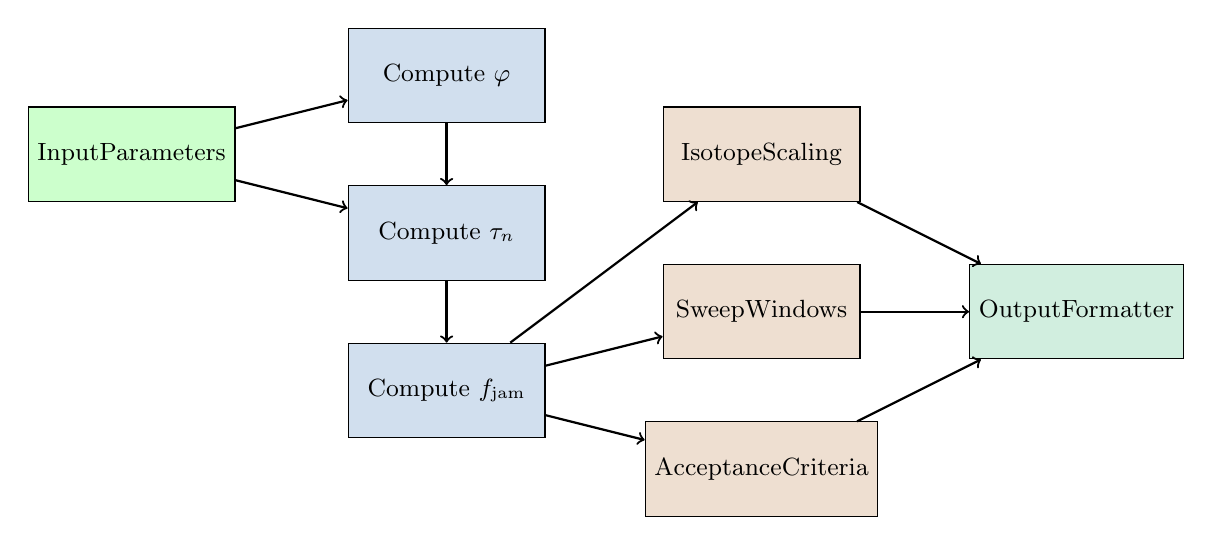
\begin{tikzpicture}[
    block/.style={rectangle, draw, minimum width=2.5cm, minimum height=1.2cm, text centered, font=\small},
    arrow/.style={->, thick}
]
    % Input
    \node[block, fill=green!20] (input) at (0,3) {Input\\Parameters};
    
    % Core computation
    \node[block, fill=compute!30] (phi) at (4,4) {Compute $\varphi$};
    \node[block, fill=compute!30] (tau) at (4,2) {Compute $\tau_n$};
    \node[block, fill=compute!30] (freq) at (4,0) {Compute $f_{\text{jam}}$};
    
    % Extended computation
    \node[block, fill=output!30] (isotope) at (8,3) {Isotope\\Scaling};
    \node[block, fill=output!30] (sweep) at (8,1) {Sweep\\Windows};
    \node[block, fill=output!30] (criteria) at (8,-1) {Acceptance\\Criteria};
    
    % Output
    \node[block, fill=validate!30] (output) at (12,1) {Output\\Formatter};
    
    % Arrows
    \draw[arrow] (input) -- (phi);
    \draw[arrow] (input) -- (tau);
    \draw[arrow] (phi) -- (tau);
    \draw[arrow] (tau) -- (freq);
    \draw[arrow] (freq) -- (isotope);
    \draw[arrow] (freq) -- (sweep);
    \draw[arrow] (freq) -- (criteria);
    \draw[arrow] (isotope) -- (output);
    \draw[arrow] (sweep) -- (output);
    \draw[arrow] (criteria) -- (output);
    
\end{tikzpicture}
\caption{System architecture for jamming frequency computation}
\label{fig:architecture}
\end{figure}

\subsubsection{Implementation Platforms}

The method may be implemented on:

\begin{enumerate}[label=(\arabic*)]
\item \textbf{General-purpose computer:} Desktop or laptop running Python, C++, MATLAB, or other scientific computing environment.

\item \textbf{Embedded controller:} Microcontroller or FPGA integrated into irradiation apparatus.

\item \textbf{Cloud computing platform:} Web service providing frequency computation as API.

\item \textbf{Mobile device:} Smartphone or tablet application for field use.

\item \textbf{Laboratory information management system (LIMS):} Integration with laboratory workflow software.
\end{enumerate}

\subsection{Input Parameters}

\subsubsection{Required Parameters}

\begin{table}[h]
\centering
\begin{tabular}{llll}
\toprule
\textbf{Parameter} & \textbf{Symbol} & \textbf{Default Value} & \textbf{Units} \\
\midrule
Rung number & $n$ & 19 & dimensionless \\
Fundamental timescale & $\tau_0$ & $7.33 \times 10^{-15}$ & seconds \\
\bottomrule
\end{tabular}
\caption{Required input parameters}
\end{table}

\subsubsection{Optional Parameters}

\begin{table}[h]
\centering
\begin{tabular}{llll}
\toprule
\textbf{Parameter} & \textbf{Symbol} & \textbf{Default Value} & \textbf{Description} \\
\midrule
Include isotope shift & --- & true & Compute D$_2$O frequency \\
Sweep margin & $\Delta f$ & 2 GHz & Window around $f_{\text{jam}}$ \\
Tolerance & $\epsilon$ & 5\% & Acceptance tolerance \\
Output format & --- & JSON & Output file format \\
Unit system & --- & GHz & Frequency units \\
\bottomrule
\end{tabular}
\caption{Optional input parameters}
\end{table}

\subsubsection{Derived Input: Fundamental Timescale}

The fundamental timescale $\tau_0$ can be computed from Planck's constant:

\begin{equation}
\tau_0 = \frac{\hbar}{E_{\text{coh}}}
\label{eq:tau0}
\end{equation}

where $E_{\text{coh}} = \varphi^{-5}$ in natural units (with appropriate conversion factors). For practical use, the default value $\tau_0 = 7.33 \times 10^{-15}$ s is recommended.

\subsection{Core Computation}

\subsubsection{Step 1: Compute Golden Ratio}

\begin{equation}
\varphi = \frac{1 + \sqrt{5}}{2} = 1.6180339887...
\label{eq:phi}
\end{equation}

Implementation note: Use extended precision (64-bit or 128-bit floating point) to maintain accuracy through subsequent power operations.

\subsubsection{Step 2: Compute Rung Timescale}

\begin{equation}
\tau_n = \tau_0 \times \varphi^n
\label{eq:tau_n}
\end{equation}

For the default rung $n = 19$:
\begin{equation}
\tau_{19} = 7.33 \times 10^{-15} \times (1.618...)^{19} \approx 6.82 \times 10^{-11} \text{ s} = 68.2 \text{ ps}
\label{eq:tau19_calc}
\end{equation}

\subsubsection{Step 3: Compute Jamming Frequency}

\begin{equation}
f_{\text{jam}} = \frac{1}{\tau_n}
\label{eq:fjam}
\end{equation}

For rung 19:
\begin{equation}
f_{\text{jam}} = \frac{1}{68.2 \times 10^{-12}} \approx 14.66 \times 10^9 \text{ Hz} = 14.66 \text{ GHz}
\label{eq:fjam_calc}
\end{equation}

\begin{figure}[h]
\centering
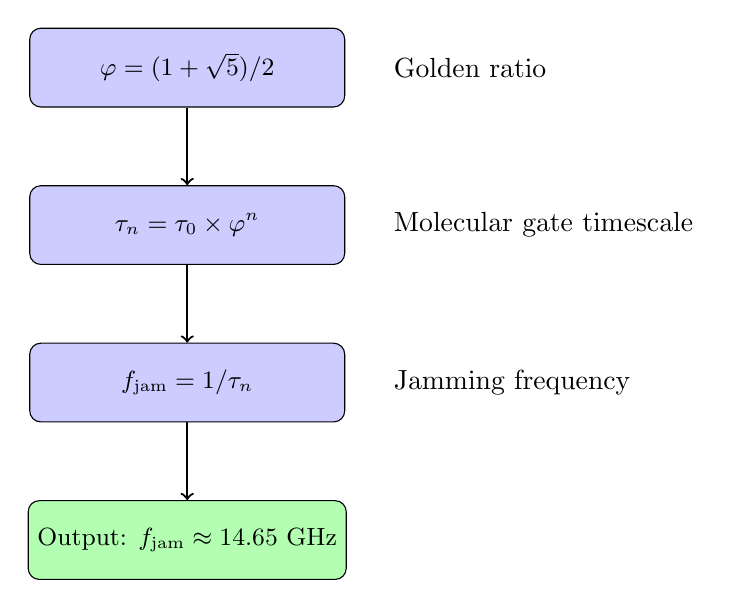
\begin{tikzpicture}[
    block/.style={rectangle, draw, rounded corners, minimum width=4cm, minimum height=1cm, text centered, font=\small},
    arrow/.style={->, thick}
]
    % Steps
    \node[block, fill=blue!20] (step1) at (0,6) {$\varphi = (1 + \sqrt{5})/2$};
    \node[block, fill=blue!20] (step2) at (0,4) {$\tau_n = \tau_0 \times \varphi^n$};
    \node[block, fill=blue!20] (step3) at (0,2) {$f_{\text{jam}} = 1/\tau_n$};
    \node[block, fill=green!30] (result) at (0,0) {Output: $f_{\text{jam}} \approx 14.65$ GHz};
    
    % Arrows
    \draw[arrow] (step1) -- (step2);
    \draw[arrow] (step2) -- (step3);
    \draw[arrow] (step3) -- (result);
    
    % Labels
    \node[right] at (2.5,6) {Golden ratio};
    \node[right] at (2.5,4) {Molecular gate timescale};
    \node[right] at (2.5,2) {Jamming frequency};
    
\end{tikzpicture}
\caption{Core computation flowchart}
\label{fig:flowchart}
\end{figure}

\subsection{Extended Computations}

\subsubsection{Isotope-Shifted Frequency}

When D$_2$O operation is required:

\begin{equation}
f_{\text{D}_2\text{O}} = \frac{f_{\text{jam}}}{\sqrt{2}} \approx 0.7071 \times f_{\text{jam}}
\label{eq:isotope}
\end{equation}

For the default jamming frequency:
\begin{equation}
f_{\text{D}_2\text{O}} = \frac{14.66}{1.414} \approx 10.37 \text{ GHz}
\label{eq:d2o_calc}
\end{equation}

\subsubsection{Frequency Sweep Windows}

Generate sweep windows for experimental validation:

\begin{align}
f_{\text{min}}^{\text{H}_2\text{O}} &= f_{\text{jam}} - \Delta f \\
f_{\text{max}}^{\text{H}_2\text{O}} &= f_{\text{jam}} + \Delta f \\
f_{\text{min}}^{\text{D}_2\text{O}} &= f_{\text{D}_2\text{O}} - \Delta f / \sqrt{2} \\
f_{\text{max}}^{\text{D}_2\text{O}} &= f_{\text{D}_2\text{O}} + \Delta f / \sqrt{2}
\end{align}

For default parameters ($\Delta f = 2$ GHz):

\begin{table}[h]
\centering
\begin{tabular}{lcc}
\toprule
\textbf{Solvent} & \textbf{$f_{\text{min}}$ (GHz)} & \textbf{$f_{\text{max}}$ (GHz)} \\
\midrule
H$_2$O & 12.66 & 16.66 \\
D$_2$O & 8.95 & 11.78 \\
\bottomrule
\end{tabular}
\caption{Computed sweep windows}
\end{table}

\subsubsection{Operating Setpoints}

Generate setpoints for irradiation apparatus:

\begin{center}
\textbf{Algorithm 3: Generate Operating Setpoints}
\end{center}
\begin{lstlisting}[frame=single]
FUNCTION GenerateSetpoints(f_jam, f_D2O, mode):
    setpoints = {}
    IF mode = "H2O" THEN
        setpoints.frequency = f_jam
        setpoints.sweep_start = f_jam - 2
        setpoints.sweep_stop = f_jam + 2
    ELSE IF mode = "D2O" THEN
        setpoints.frequency = f_D2O
        setpoints.sweep_start = f_D2O - 1.5
        setpoints.sweep_stop = f_D2O + 1.5
    END IF
    setpoints.power = 1.0          // Default power in Watts
    setpoints.temp_target = 25.0   // Default temperature
    setpoints.temp_tolerance = 0.1
    RETURN setpoints
END FUNCTION
\end{lstlisting}

\subsubsection{Acceptance Criteria}

Generate criteria for validating experimental results:

\begin{center}
\textbf{Algorithm 4: Generate Acceptance Criteria}
\end{center}
\begin{lstlisting}[frame=single]
FUNCTION GenerateAcceptanceCriteria(f_jam, f_D2O, epsilon):
    criteria = {}
    criteria.f_h2o_min = f_jam * (1 - epsilon)
    criteria.f_h2o_max = f_jam * (1 + epsilon)
    criteria.f_d2o_min = f_D2O * (1 - epsilon)
    criteria.f_d2o_max = f_D2O * (1 + epsilon)
    criteria.ratio_min = sqrt(2) * (1 - epsilon)
    criteria.ratio_max = sqrt(2) * (1 + epsilon)
    criteria.modulation_threshold = 0.10  // 10% minimum
    RETURN criteria
END FUNCTION
\end{lstlisting}

\subsection{Rung Selection}

\subsubsection{Default Rung: Molecular Gate (n=19)}

For protein folding applications, the default rung is $n = 19$, corresponding to the molecular gate timescale. This rung is selected because:

\begin{enumerate}[label=(\arabic*)]
\item It falls uniquely in the 50--100 ps window relevant to backbone dihedral transitions.
\item It corresponds to a frequency (14.65 GHz) accessible with standard microwave equipment.
\item It has been validated by machine-verified proofs.
\end{enumerate}

\subsubsection{Alternative Rungs}

The method may compute frequencies for alternative rungs:

\begin{table}[h]
\centering
\begin{tabular}{cccl}
\toprule
\textbf{Rung $n$} & \textbf{$\tau_n$ (s)} & \textbf{$f_n$ (Hz)} & \textbf{Application} \\
\midrule
15 & $3.1 \times 10^{-12}$ & 320 GHz & Fast vibrations \\
17 & $8.1 \times 10^{-12}$ & 123 GHz & Side chain dynamics \\
19 & $6.8 \times 10^{-11}$ & 14.7 GHz & Molecular gate (default) \\
21 & $1.8 \times 10^{-10}$ & 5.6 GHz & Loop motions \\
23 & $4.7 \times 10^{-10}$ & 2.1 GHz & Domain motions \\
\bottomrule
\end{tabular}
\caption{Frequencies for alternative rungs of the $\varphi$-ladder}
\end{table}

\subsection{Output Formats}

\subsubsection{JSON Output}

\begin{lstlisting}[language=Python, caption=Example JSON output]
{
  "computed_at": "2026-01-17T12:00:00Z",
  "parameters": {
    "rung": 19,
    "tau0_s": 7.33e-15,
    "phi": 1.6180339887
  },
  "frequencies": {
    "f_jam_hz": 14.66e9,
    "f_jam_ghz": 14.66,
    "f_d2o_hz": 10.37e9,
    "f_d2o_ghz": 10.37,
    "ratio": 1.414
  },
  "sweep_windows": {
    "h2o": {"min_ghz": 12.66, "max_ghz": 16.66},
    "d2o": {"min_ghz": 8.95, "max_ghz": 11.78}
  },
  "acceptance_criteria": {
    "f_h2o_range_ghz": [13.93, 15.39],
    "f_d2o_range_ghz": [9.85, 10.89],
    "ratio_range": [1.343, 1.485],
    "modulation_threshold": 0.10
  }
}
\end{lstlisting}

\subsubsection{Instrument Control File}

\begin{lstlisting}[caption=Example instrument control file]
# Jamming Frequency Control File
# Generated by Recognition Science Frequency Calculator
# Date: 2026-01-17

[FREQUENCY]
mode = fixed
frequency_ghz = 14.66
tolerance_ghz = 0.01

[SWEEP]
enabled = true
start_ghz = 12.66
stop_ghz = 16.66
step_ghz = 0.1

[POWER]
power_w = 1.0
mode = continuous

[TEMPERATURE]
target_c = 25.0
tolerance_c = 0.1

[ISOTOPE]
mode = H2O
d2o_frequency_ghz = 10.37
\end{lstlisting}

\subsubsection{CSV Output}

\begin{lstlisting}[caption=Example CSV output]
parameter,value,unit
f_jam,14.66,GHz
f_d2o,10.37,GHz
tau_19,68.2,ps
phi,1.6180339887,dimensionless
sweep_h2o_min,12.66,GHz
sweep_h2o_max,16.66,GHz
sweep_d2o_min,8.95,GHz
sweep_d2o_max,11.78,GHz
\end{lstlisting}

\subsection{Validation Integration}

\subsubsection{Pre-Experiment Validation}

Before conducting experiments, the method can validate apparatus settings:

\begin{center}
\textbf{Algorithm 5: Validate Apparatus Settings}
\end{center}
\begin{lstlisting}[frame=single]
FUNCTION ValidateSettings(settings, computed):
    errors = []
    IF |settings.frequency - computed.f_jam| > 0.5 THEN
        errors.append("Frequency out of range")
    END IF
    IF settings.temp_tolerance > 0.5 THEN
        errors.append("Temperature tolerance too large")
    END IF
    IF settings.power < 0.1 OR settings.power > 10 THEN
        errors.append("Power out of recommended range")
    END IF
    RETURN errors
END FUNCTION
\end{lstlisting}

\subsubsection{Post-Experiment Validation}

After experiments, validate results against acceptance criteria:

\begin{center}
\textbf{Algorithm 6: Validate Experimental Results}
\end{center}
\begin{lstlisting}[frame=single]
FUNCTION ValidateResults(results, criteria):
    status = "PASS"
    IF results.f_optimal < criteria.f_min OR 
       results.f_optimal > criteria.f_max THEN
        status = "FAIL: Frequency out of range"
    END IF
    IF results.modulation < criteria.modulation_threshold THEN
        status = "FAIL: Insufficient modulation"
    END IF
    IF |results.ratio - sqrt(2)| > criteria.ratio_tolerance THEN
        status = "FAIL: Isotope ratio incorrect"
    END IF
    RETURN status
END FUNCTION
\end{lstlisting}

\subsection{Implementation Examples}

\subsubsection{Python Implementation}

\begin{lstlisting}[language=Python, caption=Python implementation of core algorithm]
import math
import json

def compute_jamming_frequency(n=19, tau0=7.33e-15):
    """
    Compute jamming frequency from first principles.
    
    Args:
        n: Rung number (default 19 for molecular gate)
        tau0: Fundamental timescale in seconds
    
    Returns:
        Dictionary with computed frequencies and parameters
    """
    # Golden ratio
    phi = (1 + math.sqrt(5)) / 2
    
    # Rung timescale
    tau_n = tau0 * (phi ** n)
    
    # Jamming frequency
    f_jam = 1 / tau_n
    
    # Isotope-shifted frequency
    f_d2o = f_jam / math.sqrt(2)
    
    return {
        'phi': phi,
        'tau_n_s': tau_n,
        'f_jam_hz': f_jam,
        'f_jam_ghz': f_jam / 1e9,
        'f_d2o_hz': f_d2o,
        'f_d2o_ghz': f_d2o / 1e9,
        'ratio': math.sqrt(2)
    }

# Example usage
result = compute_jamming_frequency()
print(json.dumps(result, indent=2))
\end{lstlisting}

\subsubsection{C Implementation}

\begin{lstlisting}[language=C, caption=C implementation for embedded systems]
#include <math.h>

typedef struct {
    double phi;
    double tau_n;
    double f_jam_hz;
    double f_jam_ghz;
    double f_d2o_hz;
    double f_d2o_ghz;
} FrequencyResult;

FrequencyResult compute_jamming_frequency(int n, double tau0) {
    FrequencyResult result;
    
    // Golden ratio
    result.phi = (1.0 + sqrt(5.0)) / 2.0;
    
    // Rung timescale
    result.tau_n = tau0 * pow(result.phi, (double)n);
    
    // Jamming frequency
    result.f_jam_hz = 1.0 / result.tau_n;
    result.f_jam_ghz = result.f_jam_hz / 1.0e9;
    
    // Isotope-shifted frequency
    result.f_d2o_hz = result.f_jam_hz / sqrt(2.0);
    result.f_d2o_ghz = result.f_d2o_hz / 1.0e9;
    
    return result;
}
\end{lstlisting}

\subsection{API Specification}

\subsubsection{REST API Endpoint}

\begin{lstlisting}[caption=REST API specification]
POST /api/v1/compute-frequency

Request Body:
{
  "rung": 19,                    // Optional, default 19
  "tau0": 7.33e-15,              // Optional, default value
  "include_isotope": true,       // Optional, default true
  "sweep_margin_ghz": 2.0,       // Optional, default 2.0
  "tolerance": 0.05,             // Optional, default 0.05
  "output_format": "json"        // Optional: json, csv, instrument
}

Response:
{
  "status": "success",
  "data": {
    "frequencies": {...},
    "sweep_windows": {...},
    "acceptance_criteria": {...},
    "setpoints": {...}
  }
}
\end{lstlisting}

\subsection{Error Handling}

The method includes error handling for:

\begin{enumerate}[label=(\arabic*)]
\item \textbf{Invalid rung number:} Rung must be positive integer.
\item \textbf{Invalid $\tau_0$:} Must be positive and physically reasonable.
\item \textbf{Numerical overflow:} Large rung numbers may exceed floating-point range.
\item \textbf{Output formatting errors:} Invalid format specifications.
\end{enumerate}

\newpage

%% ============================================================================
%%                              CLAIMS
%% ============================================================================

\section{CLAIMS}

What is claimed is:

\subsection{Core Computation Claims}

\begin{enumerate}[label=\textbf{\arabic*.}]

\item A computer-implemented method for calculating a frequency for modulating protein folding, comprising:
\begin{enumerate}[label=(\alph*)]
\item receiving, by a processor, input parameters including a rung number $n$ and a fundamental timescale $\tau_0$;
\item computing, by the processor, the golden ratio $\varphi = (1+\sqrt{5})/2$;
\item computing, by the processor, a molecular gate timescale $\tau_n = \tau_0 \times \varphi^n$;
\item computing, by the processor, a jamming frequency $f_{\text{jam}} = 1/\tau_n$; and
\item outputting, by the processor, the jamming frequency in a machine-readable format.
\end{enumerate}

\item The method of claim 1, wherein the rung number $n$ is 19 and the fundamental timescale $\tau_0$ is approximately $7.33 \times 10^{-15}$ seconds.

\item The method of claim 1, wherein the jamming frequency is approximately 14.65 GHz.

\item The method of claim 1, further comprising computing an isotope-shifted frequency $f_{\text{D}_2\text{O}} = f_{\text{jam}}/\sqrt{2}$.

\item The method of claim 4, wherein the isotope-shifted frequency is approximately 10.37 GHz.

\item The method of claim 1, wherein the machine-readable format is selected from JSON, CSV, XML, and instrument control file format.

\end{enumerate}

\subsection{Setpoint Generation Claims}

\begin{enumerate}[label=\textbf{\arabic*.}]
\setcounter{enumi}{6}

\item A computer-implemented method for generating operating setpoints for a protein folding modulation apparatus, comprising:
\begin{enumerate}[label=(\alph*)]
\item computing a jamming frequency according to claim 1;
\item generating a frequency setpoint equal to the computed jamming frequency;
\item generating a frequency sweep window comprising a minimum frequency and a maximum frequency centered on the jamming frequency;
\item generating a power setpoint;
\item generating a temperature setpoint and temperature tolerance; and
\item outputting the setpoints in a format compatible with the apparatus.
\end{enumerate}

\item The method of claim 7, wherein the frequency sweep window spans from $(f_{\text{jam}} - \Delta f)$ to $(f_{\text{jam}} + \Delta f)$, where $\Delta f$ is a configurable sweep margin.

\item The method of claim 7, further comprising generating setpoints for D$_2$O operation by scaling the frequency setpoint and sweep window by factor $1/\sqrt{2}$.

\item The method of claim 7, wherein the output format is an instrument control file comprising frequency, power, and temperature parameters.

\end{enumerate}

\subsection{Acceptance Criteria Claims}

\begin{enumerate}[label=\textbf{\arabic*.}]
\setcounter{enumi}{10}

\item A computer-implemented method for generating acceptance criteria for validating protein folding modulation experiments, comprising:
\begin{enumerate}[label=(\alph*)]
\item computing a jamming frequency and isotope-shifted frequency according to claims 1 and 4;
\item computing a frequency acceptance range for H$_2$O experiments as $(f_{\text{jam}} \times (1-\epsilon), f_{\text{jam}} \times (1+\epsilon))$;
\item computing a frequency acceptance range for D$_2$O experiments as $(f_{\text{D}_2\text{O}} \times (1-\epsilon), f_{\text{D}_2\text{O}} \times (1+\epsilon))$;
\item computing a frequency ratio acceptance range as $(\sqrt{2} \times (1-\epsilon), \sqrt{2} \times (1+\epsilon))$;
\item setting a modulation threshold; and
\item outputting the acceptance criteria.
\end{enumerate}

\item The method of claim 11, wherein $\epsilon$ is 5\%.

\item The method of claim 11, wherein the modulation threshold is 10\%.

\item A computer-implemented method for validating experimental results against computed acceptance criteria, comprising:
\begin{enumerate}[label=(\alph*)]
\item receiving experimental results including observed optimal frequency and observed modulation;
\item receiving acceptance criteria generated according to claim 11;
\item comparing the observed optimal frequency to the frequency acceptance range;
\item comparing the observed modulation to the modulation threshold;
\item outputting a validation status of PASS if all comparisons are within criteria, or FAIL with a reason if any comparison is outside criteria.
\end{enumerate}

\end{enumerate}

\subsection{System Claims}

\begin{enumerate}[label=\textbf{\arabic*.}]
\setcounter{enumi}{14}

\item A system for computing protein folding jamming frequencies, comprising:
\begin{enumerate}[label=(\alph*)]
\item a processor;
\item a memory storing instructions that, when executed by the processor, cause the processor to perform the method of claim 1;
\item an input interface for receiving computation parameters; and
\item an output interface for delivering computed frequencies and related parameters.
\end{enumerate}

\item The system of claim 15, wherein the system is implemented as a cloud computing service accessible via API.

\item The system of claim 15, wherein the system is implemented as embedded firmware in a protein folding modulation apparatus.

\item The system of claim 15, wherein the system is implemented as a mobile application.

\end{enumerate}

\subsection{Integration Claims}

\begin{enumerate}[label=\textbf{\arabic*.}]
\setcounter{enumi}{18}

\item A method for controlling a protein folding modulation apparatus using computed frequencies, comprising:
\begin{enumerate}[label=(\alph*)]
\item computing a jamming frequency according to claim 1;
\item transmitting the computed frequency to a frequency controller of the apparatus;
\item commanding the apparatus to irradiate a sample at the computed frequency; and
\item receiving measurement data from the apparatus.
\end{enumerate}

\item The method of claim 19, further comprising:
\begin{enumerate}[label=(\alph*)]
\item generating acceptance criteria according to claim 11;
\item validating the measurement data against the acceptance criteria; and
\item outputting a validation report.
\end{enumerate}

\item A non-transitory computer-readable medium storing instructions that, when executed by a processor, cause the processor to perform the method of claim 1.

\item The non-transitory computer-readable medium of claim 21, further storing instructions to perform the methods of claims 7 and 11.

\end{enumerate}

\newpage

%% ============================================================================
%%                         ABSTRACT
%% ============================================================================

\section*{ABSTRACT}
\addcontentsline{toc}{section}{ABSTRACT}

A computer-implemented method for calculating the frequency for modulating protein folding rates from first principles. The method comprises: computing the golden ratio $\varphi = (1+\sqrt{5})/2$; computing a molecular gate timescale $\tau_n = \tau_0 \times \varphi^n$ for a selected rung number $n$ (default $n=19$); computing a jamming frequency $f_{\text{jam}} = 1/\tau_n$ (approximately 14.65 GHz); optionally computing an isotope-shifted frequency $f_{\text{D}_2\text{O}} = f_{\text{jam}}/\sqrt{2}$ (approximately 10.37 GHz); and outputting the computed values. The method further generates operating setpoints for irradiation apparatus, frequency sweep windows for experimental validation, and acceptance criteria for result validation including frequency ranges, frequency ratios, and modulation thresholds. The method may be implemented on general-purpose computers, embedded controllers, cloud platforms, or mobile devices, with outputs in JSON, CSV, instrument control file, or other formats. The method implements the Recognition Science framework for deriving physical constants from the golden ratio, with underlying derivations verified by machine-checked proofs. Applications include controlling protein folding modulation apparatus, validating experimental results, and providing computational support for research and industrial applications.

\vspace{1in}

\begin{center}
\textbf{--- END OF SPECIFICATION ---}
\end{center}

\newpage

%% ============================================================================
%%                         INVENTOR DECLARATION
%% ============================================================================

\section*{INVENTOR DECLARATION}
\addcontentsline{toc}{section}{INVENTOR DECLARATION}

I, Jonathan Washburn, declare that:

\begin{enumerate}[label=(\arabic*)]
\item I am the original and sole inventor of the computer-implemented method described and claimed in this application.

\item I have reviewed the above specification and claims and believe them to be accurate and complete.

\item I believe the claimed invention to be novel, useful, and non-obvious over the prior art.

\item I authorize the filing of this provisional patent application to establish a priority date.
\end{enumerate}

\vspace{1in}

\noindent\textbf{Inventor Signature:} \hrulefill

\vspace{0.5in}

\noindent\textbf{Name:} Jonathan Washburn

\noindent\textbf{Email:} washburn.jonathan@gmail.com

\noindent\textbf{Date:} \hrulefill

\vspace{1in}

\begin{center}
\textit{This document is intended for provisional patent application filing purposes.\\
All information contained herein is confidential and proprietary.}
\end{center}

\end{document}
